\documentclass[12pt,a4paper]{article}
\usepackage[utf8]{inputenc}
\usepackage[german]{babel}
\usepackage{german}
\usepackage{siunitx}
\usepackage{hyperref,ulem,setspace}
\usepackage{caption,subcaption}
\usepackage{graphicx,pgfplots}
\pgfplotsset{compat=1.9}
\normalem

\title{Projektbericht}
\author{R. Brandis \and K. Läufer}
\date{\today}

\begin{document}
\maketitle
\newpage
\tableofcontents
\newpage

\section{Aufgabenstellung}

\section{Extern modulierter Laser}
Um mit einem mit konstanter Intensität strahlenden Laser Informationen zu übertragen, muss mindestens ein Parameter des Laserstrahls extern moduliert werden. Mögliche Modulationsparameter sind beispielsweise die Amplitude oder die Phase des Strahls. In unseren Versuchen kam ausschließlich Amplitudenmodulation zum Einsatz.

Wenn die Amplitude eines Laserstrahls extern moduliert werden soll, sind wiederum verschiedene Aufbauten als Modulator denkbar. Ein Lautsprecher mit einem in der Mitte der Membran angebrachten kleinen Spiegel kann je nach Auslenkung der Membran die Intensität des auf der Photodiode des Empfängers auftreffenden Lichts verändern; mit dieser Technik hat sich eine zweite Projektgruppe genauer beschäftigt. Wir haben uns stattdessen für die Variante entschieden, bei der ein einzelner LCD-Pixel (engl. \textit{liquid crystal display}) zum Einsatz kommt.

\subsection{LCD-Modul als Modulator}
\begin{itemize}
\item Allgemeines Funktionsprinzip eines LCDs
\item Versuchsaufbau beschreiben
\item Resultate Übertragungsfunktion
\end{itemize}
Ein einzelner Pixel eines LCD besteht üblicherweise aus einer Flüssigkristallschicht, an die über zwei Elektroden ein elektrisches Feld angelegt werden kann, sowie einem horizontalen und einem vertikalen Polarisationsfilter, je einer vor und einer hinter der Kristallschicht.

Wären die Flüssigkristalle nicht vorhanden, würden beide Polarisationsfilter zusammen das gesamte einfallende Licht herausfiltern. Die zusätzliche Kristallschicht zwischen beiden Filtern sorgt nun für eine Drehung der Polarisation des durch den ersten Filter polarisierten Lichts. Da sich die Ausrichtung der Kristalle über das angelegte Feld bzw. über die angelegte Spannung steuern lässt, lässt sich somit auch die Menge des insgesamt durchgelassenen Lichts steuern.

Da in unseren Versuchsaufbauten eine Laserdiode als Lichtquelle diente, war das in den Modulator einfallende Licht bereits polarisiert. Der von uns verwendete LCD-Pixel musste daher nur über einen Polarisationsfilter hinter der Kristallschicht verfügen.

\subsubsection{Übertragungscharakteristik}



\begin{tikzpicture}
  \begin{semilogxaxis}[
    log ticks with fixed point,
    xlabel={Frequenz [Hz]},
    ylabel={Spannung [dB]},
    xmin=9.1,
    xmax=1200,
    ymin=0,
    ymax=65,
    width=0.94\textwidth,
    height=0.57\textwidth,
    axis x line=bottom,
    axis y line=left
  ]
  \addplot+[smooth] table [x=f, y=u_db, col sep=comma] {2.1_lcd_sweep_data.csv};
  \end{semilogxaxis}
\end{tikzpicture}


\subsection{Übertragung von Audiosignalen}
\begin{itemize}
\item Aufbau erklären
\item Unterpunkt zu Lichtempfaengerschaltungen
\end{itemize}

\subsection{Übertragung digitaler Daten}






\section{Direkt modulierter Laser}
Im zweiten Teil des Projekts sollte ein Diodenlaser direkt moduliert werden um damit digitale Daten zu übertragen. Dazu hatte die andere Gruppe bereits eine Modulationsmethode untersucht, bei der auf einen konstanten Strom ein Datensignal aufgekoppelt wurde.

Unser Ziel war es eine Stromquelle direkt mit einem Datensignal zu modulieren und danach Empfängerdesigns zu evaluieren.


\subsection{Sender: modulierte Konstantstromquelle}
\label{sec:direct_tx}
Auf Grund der exponentiellen Kennlinie einer Laserdiode muss diese mit einem konstanten Strom versorgt werden. Eine einfache Konstantstromquelle kann mit zwei Bipolartransisoren aufgebaut werden. Der Strom $I_{D1}$ , der durch die Diode fließt entspricht hierbei in etwa dem Strom $I_{R1}$, der durch den Widerstand $R1$ fließt. An diesem müssen, durch den Transistor  $Q2$ vorgegeben, etwa \SI{0.7}{\volt} abfallen, wodurch sich ungefähr folgender Strom einstellt:

\begin{equation}
I_{D1} = I_{R1} = \frac{U_{R1}}{R1} \approx \frac{\SI{0.7}{\volt}}{R1}
\end{equation}

Diese Quelle lässt sich leicht ein und aus schalten in dem - über einen Widerstand - die Kollektor-Emitter-Spannung $U_{CE2}$ des Transistor $Q2$ vorgegeben wird. Dieser Aufbau ist in Abbildung~\ref{fig:modulated_current_source} zu sehen.

\begin{figure}[!h]
  \centering
    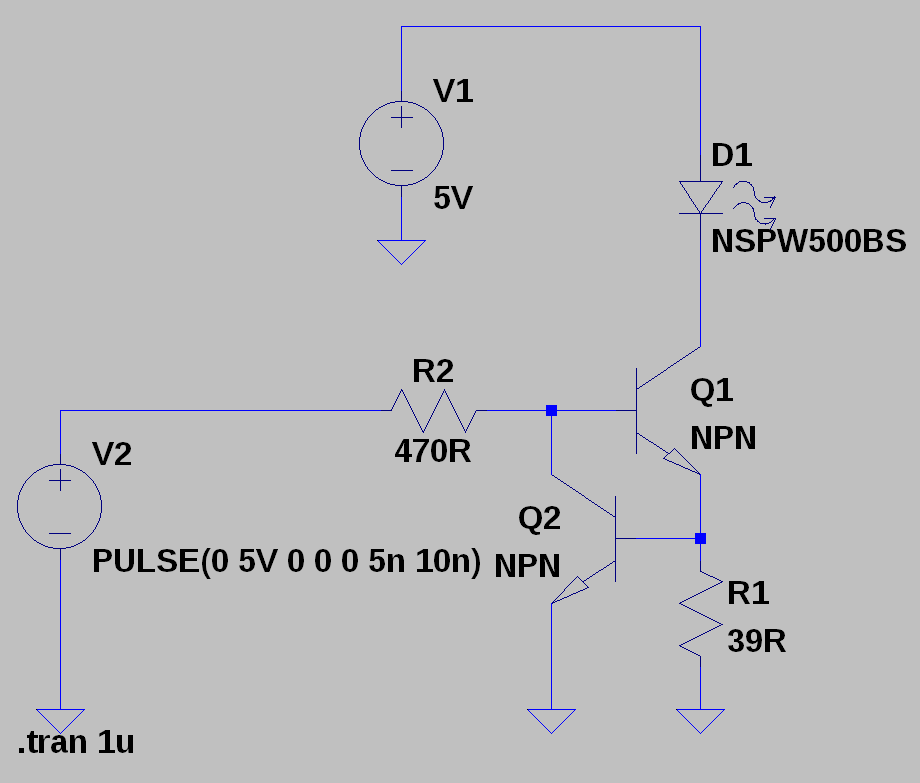
\includegraphics[width=0.8\textwidth]{../spice/modulated_current_source.png}
  \caption{Modulierte Stromquelle.}
  \label{fig:modulated_current_source}
\end{figure}

\begin{figure}[!h]
  \centering
    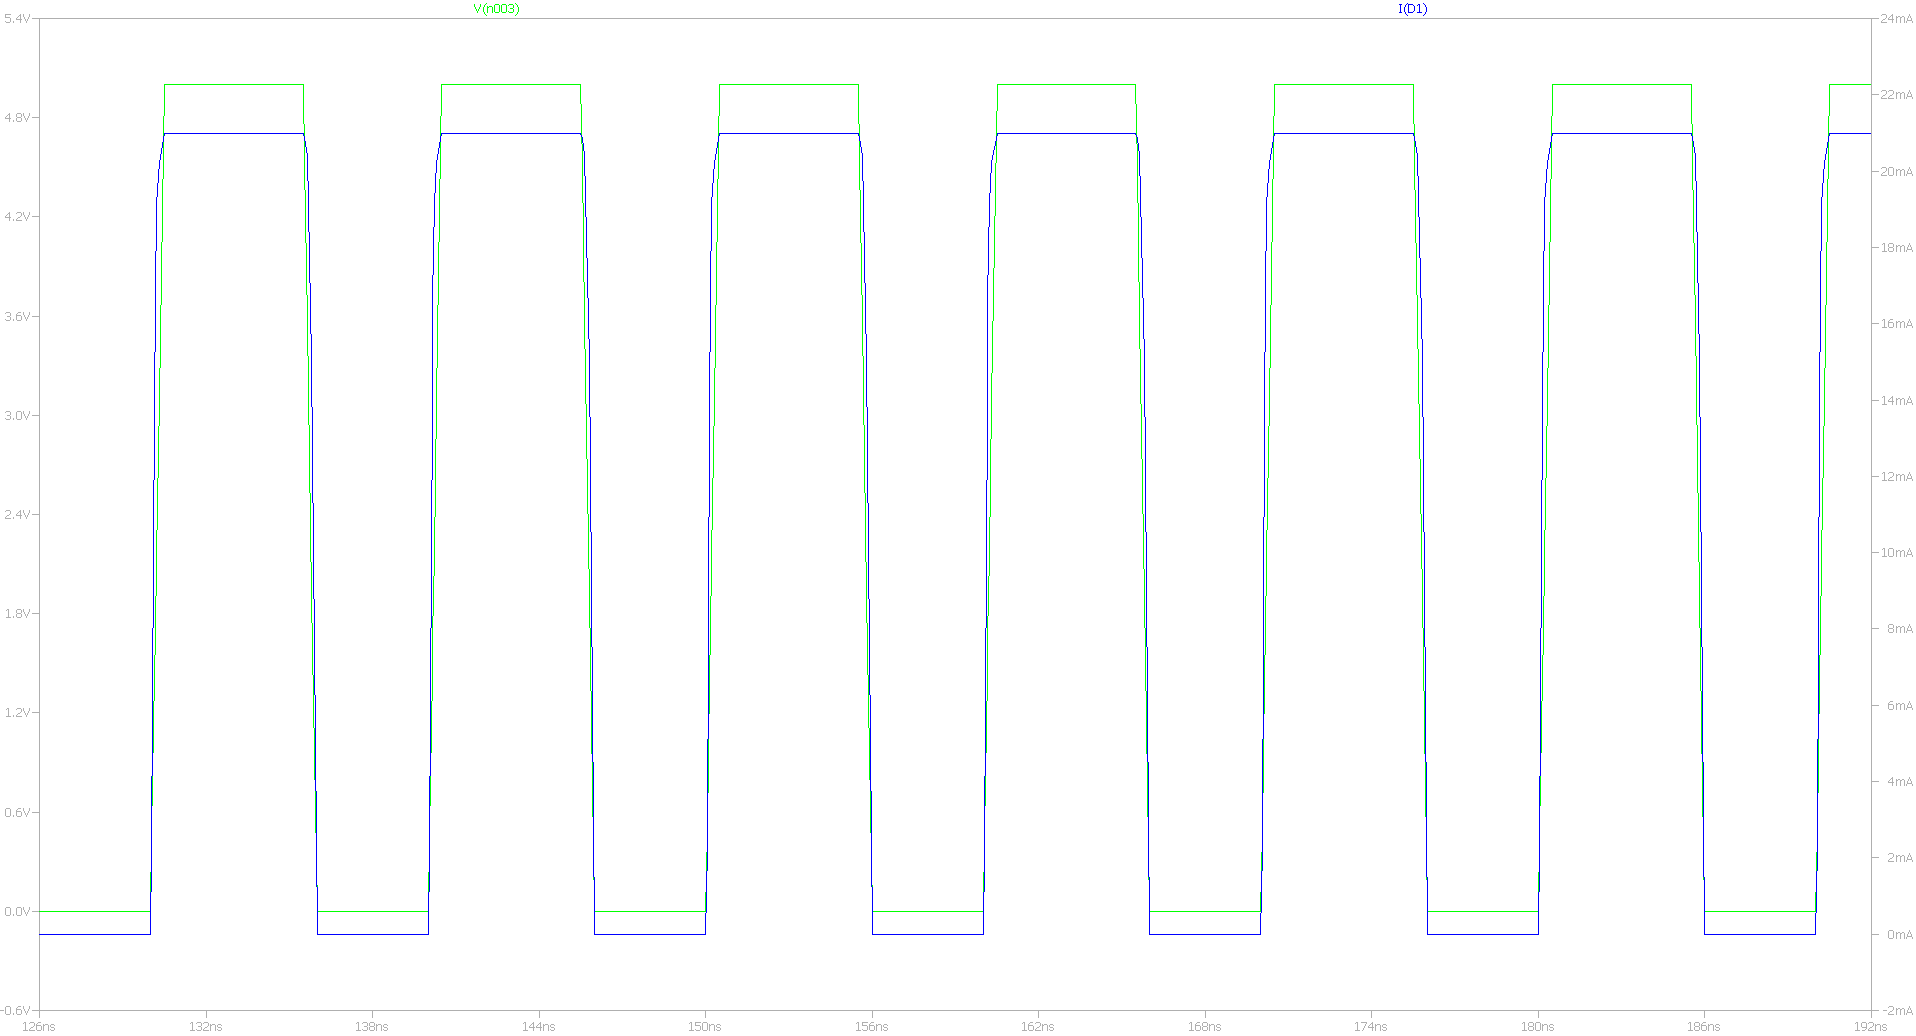
\includegraphics[width=1.0\textwidth]{../spice/current_input_v_current_out_trans.png}
  \caption{Transientenanalyse der modulierten Stromquelle.}
  \label{fig:modulated_current_source_plot}
\end{figure}


Eine Simulation des Aufbaus in LTSpice zeigt, dass der Strom $I_{D1}$ durch die Diode von der Eingangsspannung $U_2$ abhängt. Die in Abbildung~\ref{fig:modulated_current_source_plot} dargestellten Ergebnisse wurde aber mit einem vereinfachten Transistormodell simuliert, sind also mit Vorsicht zu genießen. Das Prinzip wird darin aber gut veranschaulicht.

\begin{figure}[!h]
  \centering
    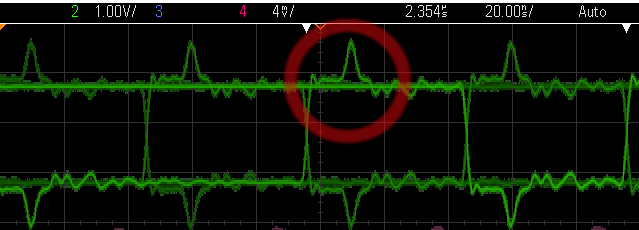
\includegraphics[width=1.0\textwidth]{img/ring_20MHz.png}
  \caption{Reflexionen bei einem \SI{20}{\mega\hertz} Eingangssignal.}
  \label{fig:ring_20mhz}
\end{figure}

Mit diesem Aufbau ließen sich recht schnelle Übertragungen von zufälligen Bits realisieren (siehe auch Abschnitt~\ref{sec:direct_rx}). Es gab jedoch, auf Grund der fehlenden Terminierung auf der Eingangsseite unserer Schaltung, Probleme mit Reflexionen auf der Leitung (siehe Abbildung~\ref{fig:ring_20mhz}). Hier wäre eine Untersuchung verschiedener Terminierungsvarianten interessant. Auch verhält sich die Schaltung bei Frequenzen im Megahertzbereich nicht genauso wie in der Simulation, so entspricht die Spannung am Widerstand $R1$ nicht den erwarteten \SI{0.7}{\volt}. Hier wären eine Verbesserung der Spice Simulation durch die Auswahl eines passenden Transistormodells und bessere Modellierung der Quelle sowie weitere empirische Versuche angebracht.

\subsection{Photodiode mit Lastwiderstand als Empfänger}
\label{sec:direct_rx}

\begin{figure}[h]
  \centering
  \begin{subfigure}[b]{0.6\textwidth}
    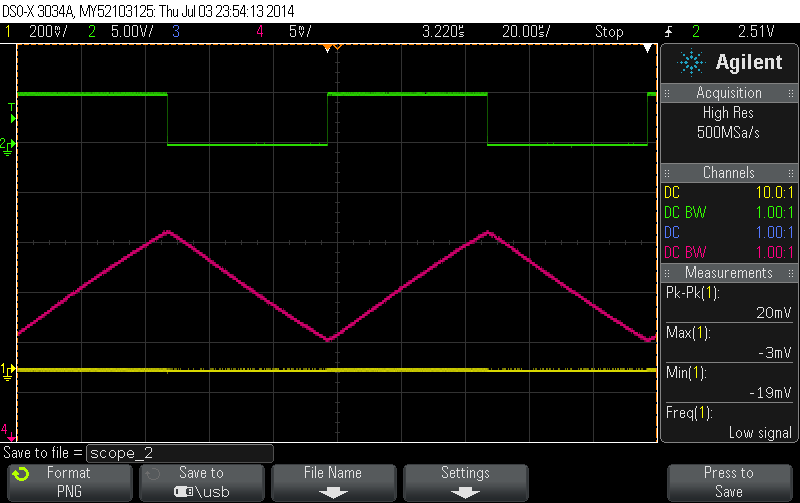
\includegraphics[width=\textwidth]{../measurements/20140703/20kHz_10kOhm/scope_2.png}
    \caption{\SI{10}{\kilo\ohm}}
    \label{fig:direct_rx_10k_R}
  \end{subfigure}  
  \begin{subfigure}[b]{0.6\textwidth}
    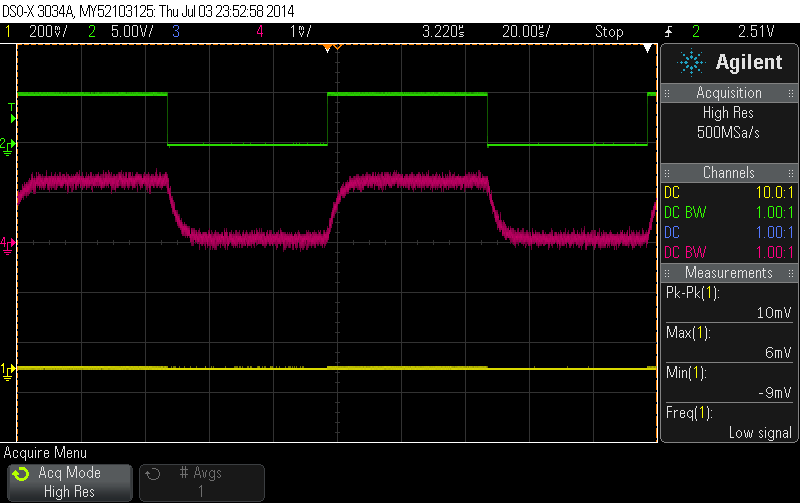
\includegraphics[width=\textwidth]{../measurements/20140703/20kHz_50_Ohm/scope_0.png}
    \caption{\SI{50}{\ohm}}
    \label{fig:direct_rx_50_R}
  \end{subfigure}  
  \caption{\SI{20}{\kilo\hertz} Eingangssignal mit unterschiedlichem Lastwiderstand}
  \label{fig:direct_rx}
\end{figure}

Als Empfänger nutzten wir zunächst, zum Testen der Sendeschaltung, eine Photodiode mit Biasspannung und umschaltbaren Lastwiderstand von ThorLabs (\textbf{??Typenbezeichnung??}).

In der Abbildung~\ref{fig:direct_rx} kann man die Abhängigkeit des Ausgangssignals vom Lastwiderstand sehen. Dazu wurde der Ausgang der Photodiode mit einem hochohmig terminierten Eingang eines Oszilloskops verbunden und auf den Eingang unserer Sendeschaltung~\ref{sec:direct_tx} ein \SI{20}{\kilo\hertz} Rechtecksignal gegeben. Bei einem hohen Lastwiderstand (\ref{fig:direct_rx_10k_R}) erhöht sich die Verstärkung: die Amplitude ist hier in etwa \SI{10}{\milli\volt}. Jedoch sinkt die Bandbreite, was sich an sehr langen Anstiegs- und Abfallzeiten und der daraus resultierenden Dreiecksform des Ausgangssignals bemerkbar macht. Mit einem kleineren Lastwiderstand (\ref{fig:direct_rx_50_R}) ergibt sich ein weniger verzerrtes Signal, die Amplitude beträgt jedoch nur noch in etwa \SI{1}{\milli\volt}.

Die kleinen Amplituden und die Verzerrung beim Empfang eines \SI{20}{\kilo\hertz} Signals weisen darauf hin, dass für schnellere Signale ein besserer Verstärker benötigt wird.

\subsection{Empfänger mit integriertem \textit{AD8015} Transimpedanzverstärker}
Anstatt selbst eine Empfängerschaltung aufzubauen, bietet es sich an, einen integrierten Transimpedanzverstärker wie den \textit{AD8015} zu benutzen. Dieser ist von Grund auf dazu konzipiert, den Photostrom in eine proportional verstärkte Spannung zu wandeln, welche differentiell mit 50 Ohm Impedanz am Ausgang abgegriffen werden kann. Dieser benötigt nur wenige externe Komponenten was zu einer einfachen Schaltung führt (\ref{fig:receiver_sch})


\begin{figure}[h]
  \centering
    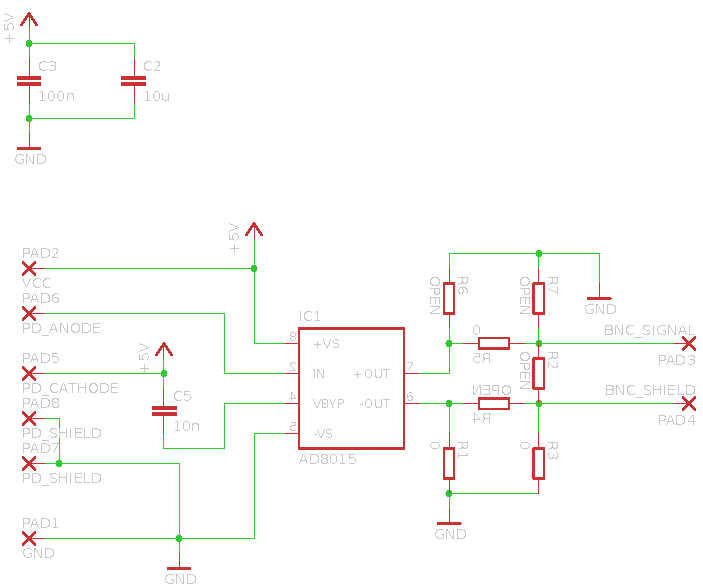
\includegraphics[width=0.7\textwidth]{img/receiver.pdf}
  \caption{Beschaltung des \textit{AD8015} Transimpedanzverstärkers}
  \label{fig:receiver_sch}
\end{figure}

Mit diesem Aufbau lassen sich auch schnelle Signale verstärken was in der Betrachtung der Augendiagramme zu sehen ist.


\subsection{Augendiagramme}
Augendiagramme können mit dem Oszilloskop aufgenommen werden. Hierzu wird der Trigger auf steigende und fallende Flanken des Signals eingestellt und Persistenz aktiviert. Hierdurch erhält man eine Überlagerung von steigenden und fallenden Flanken. Verbleibt zwischen diesen eine klar erkennbare Öffnung (das Auge), dann kann man davon ausgehen, dass die Bits auch von einer Empfängerschaltung richtig interpretiert werden können. Wichtig ist, als Eingangssignal eine Zufallssequenz von Bits zu wählen, damit sich das System nicht einfach auf eine Frequenz einschwingt.

\begin{figure}[h]
  \centering
    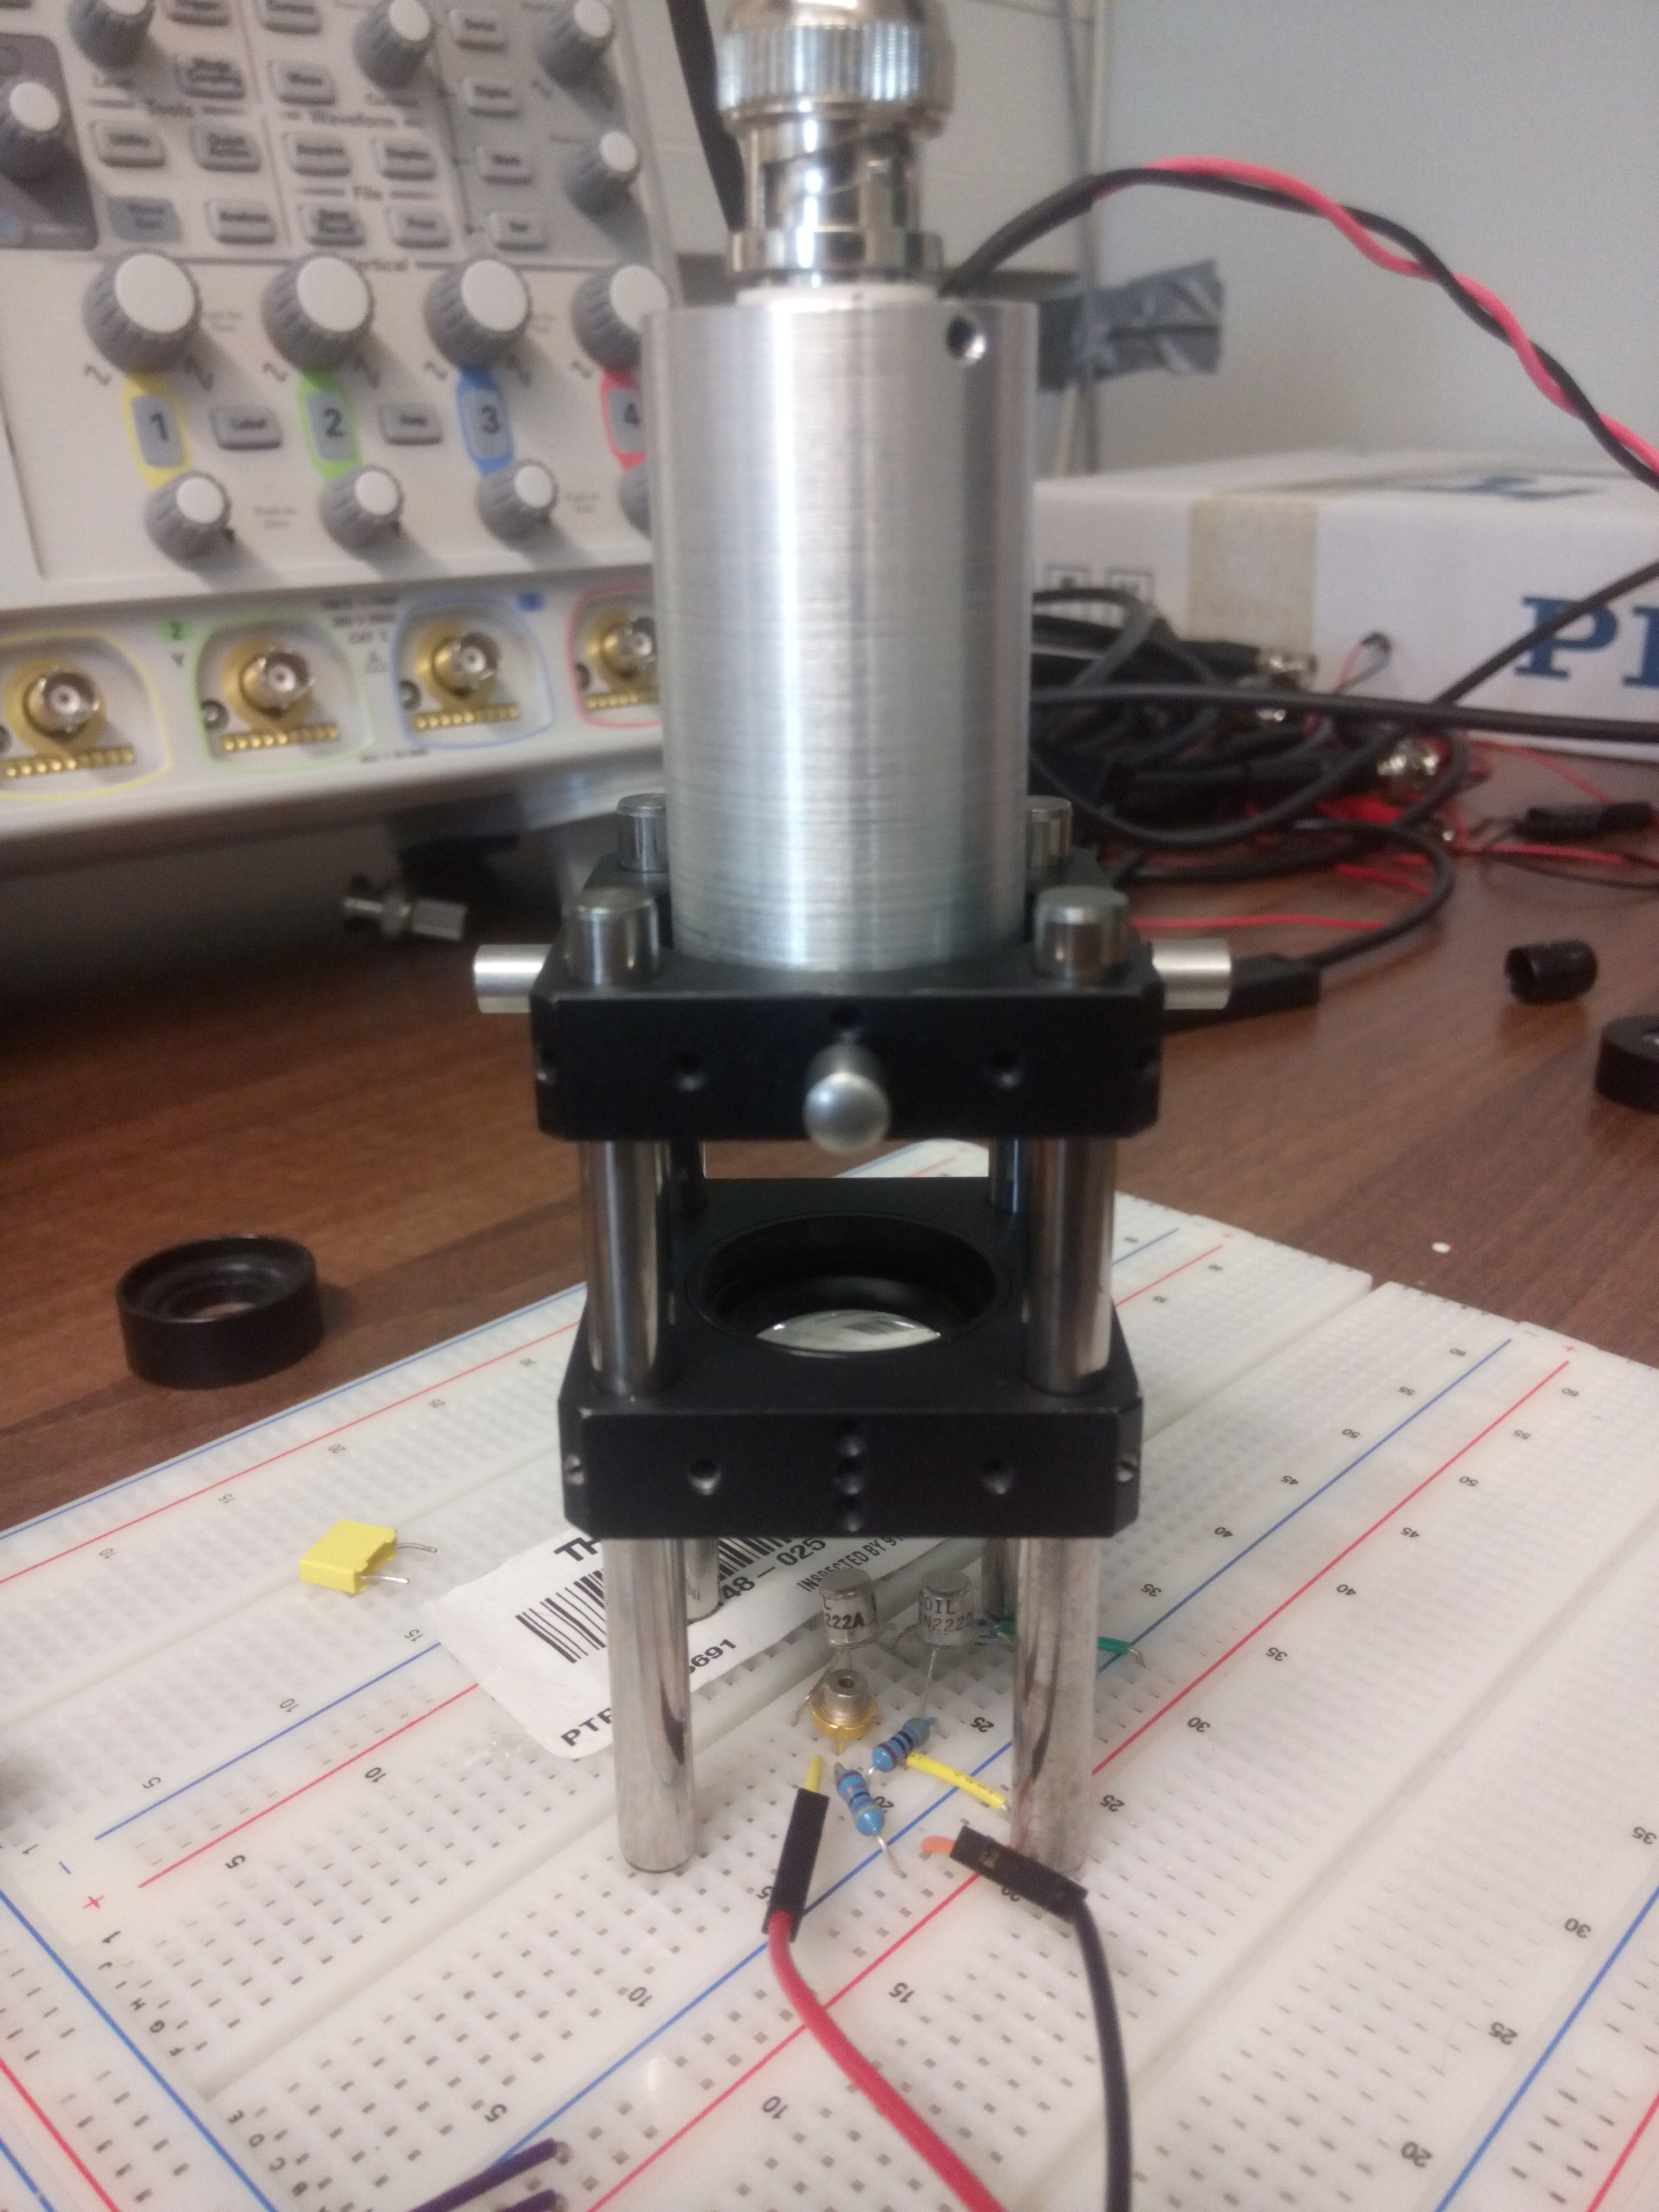
\includegraphics[width=0.7\textwidth]{../photos/IMG_20140710_184030.jpg}
  \caption{Versuchsaufbau zur Bestimmung der Augendiagramme.}
  \label{fig:eye_setup}
\end{figure}

In unserem Fall wurden die Augendiagramme in Abbildung~\ref{fig:eye_plots_slow} und Abbildung~\ref{fig:eye_plots_fast} mit der Sendeschaltung aus Abschnitt~\ref{sec:direct_tx} und der Empfängerschaltung mit dem \textit{AD8015} TIA aufgenommen. Der Aufbau ist in Abbildung~\ref{fig:eye_setup} zu sehen.

\begin{figure}[!h]
  \centering
  \begin{subfigure}[b]{0.6\textwidth}
    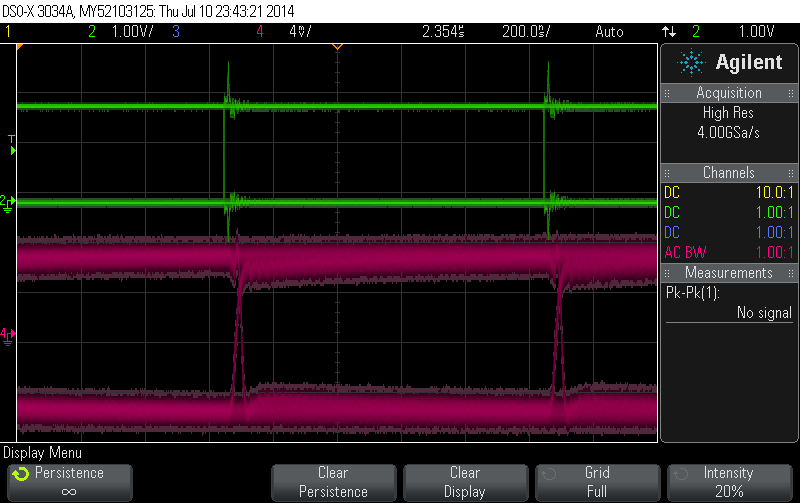
\includegraphics[width=\textwidth]{../measurements/20140710/eye_plots/01MHz.png}
    \caption{\SI{1}{\mega\hertz}}
  \end{subfigure}  
  \begin{subfigure}[b]{0.6\textwidth}
    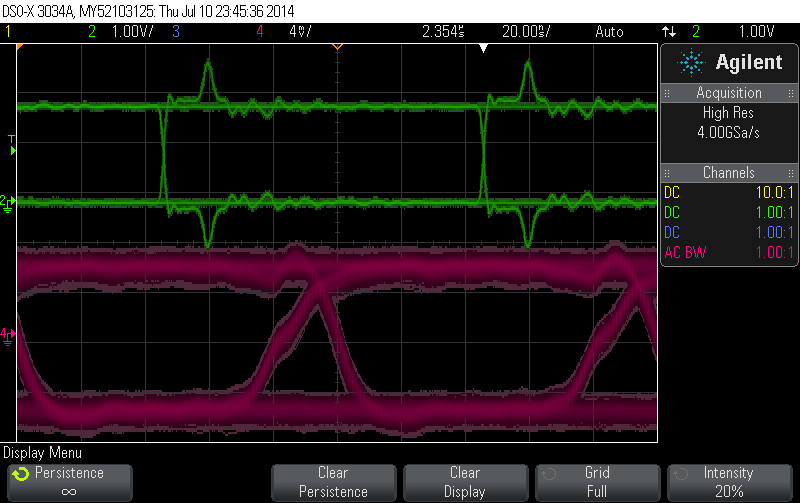
\includegraphics[width=\textwidth]{../measurements/20140710/eye_plots/10MHz.png}
    \caption{\SI{10}{\mega\hertz}}
  \end{subfigure}  
  \caption{Augendiagramme}
  \label{fig:eye_plots_slow}
\end{figure}

\begin{figure}[!h]
  \centering
  \begin{subfigure}[b]{0.6\textwidth}
    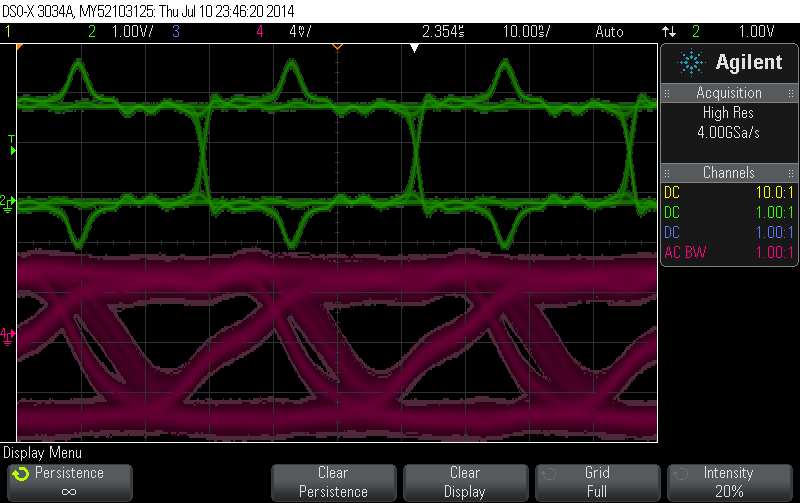
\includegraphics[width=\textwidth]{../measurements/20140710/eye_plots/30MHz.png}
    \caption{\SI{30}{\mega\hertz}}
  \end{subfigure}  
  \begin{subfigure}[b]{0.6\textwidth}
    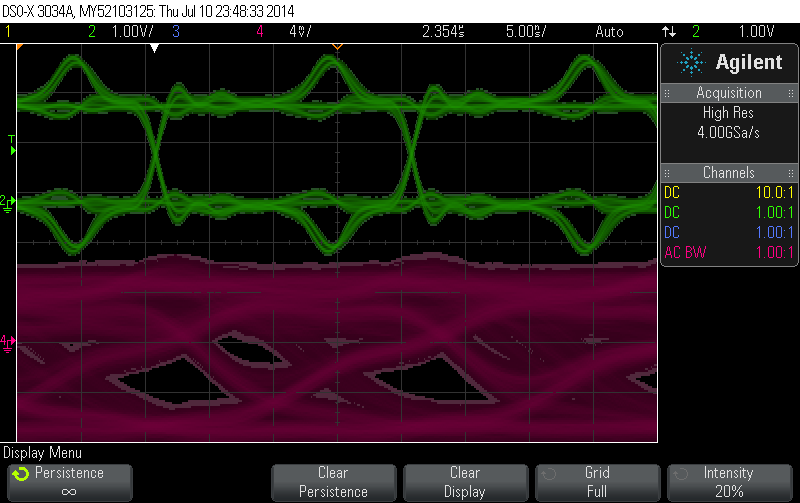
\includegraphics[width=\textwidth]{../measurements/20140710/eye_plots/50MHz.png}
    \caption{\SI{50}{\mega\hertz}}
  \end{subfigure}  
  \caption{Augendiagramme}
  \label{fig:eye_plots_fast}
\end{figure}



Ein \SI{1}{\mega\hertz} Bitsignal wird ohne Probleme übertragen, auch bei einem \SI{10}{\mega\hertz} Signal ist die Augenöffnung noch unproblematisch. Ein \SI{30}{\mega\hertz} Signal hat bereits eine deutlich kleiner Öffnung, sollte aber auch noch funktionieren. Bei einem \SI{50}{\mega\hertz} Signal scheint die Grenze erreicht; hier ist keine distinkte Öffnung mehr zu erkennen. 

\subsection{Ergebnisse}
Mit dem System aus selbst gebauter modulierbarer Stromquelle und \textit{AD8015} Verstärker lassen sich mit Signale mit einer Geschwindigkeit von bis zu \SI{50}{\mega\hertz} gut übertragen. Die Diode ohne Verstärker ist in diesem Geschwindigkeitsbereich eher nicht mehr zu gebrauchen.

Bezüglich der Sendeschaltung sollte man als nächstes versuchen, diese, wie oben genannt, zu verbessern um dann eine Platine mit dieser aufzubauen. Zusammen mit einem Gehäuse lässt sich damit ein Versuchsaufbau erstellen, mit dem die Schaltung noch besser untersucht und der Laser auch in eine Glasfaser eingekoppelt werden kann.

Der Empfänger mit \textit{AD8015} hat sich bewährt und muss wohl erst einmal nicht verändert werden. Es wäre aber interessant diesen noch besser zu vermessen. Unter anderem sollte mit einer professionellen Lichtquelle untersucht werden, bis zu welchen Frequenzen verstärkt werden kann. Bisher wurde hier nur das Gesamtsystem aus Empfänger und Sender untersucht, was es erschwert, eindeutige Aussagen über die Einzelkomponente zu machen. Interessant könnte es auch sein, die \textit{AD8015} Schaltung mit verschiedenen Photodioden aufzubauen und zu untersuchen, wie sich diese auf das Verstärkungsverhalten auswirken.

\section{Fazit}

\end{document}
